\documentclass{article}
\usepackage[margin=1in]{geometry}
\usepackage{amsmath,amsthm,amssymb}
\usepackage{bbm,enumerate,mathtools}
\usepackage{tikz,pgfplots}
\usepackage{chessboard}
\usepackage[hidelinks]{hyperref}
\usepackage{multicol} % Problem 35
\usepackage{xstring} % Difficulty command
\usetikzlibrary{shapes.geometric}

\newenvironment{question}{\begin{trivlist}\item[\textbf{Question.}]}{\end{trivlist}}
\newenvironment{note}{\begin{trivlist}\item[\textbf{Note.}]}{\end{trivlist}}
\newenvironment{references}{\begin{trivlist}\item[\textbf{References.}]}{\end{trivlist}}
\newenvironment{related}{\begin{trivlist}\item[\textbf{Related.}]\end{trivlist}\begin{enumerate}}{\end{enumerate}}

\newcommand\score[1]{
\pgfmathsetmacro\pgfxa{#1+1}
\tikzstyle{scorestars}=[
  star,
  star points=5,
  star point ratio=2.25,
  draw,
  inner sep=3pt,
  anchor=outer point 5
]
  \begin{tikzpicture}[baseline]
    \draw[opacity=0] (0,-0.5) rectangle (0,0.2); % Workaround for whitespace at the bottom.
    \foreach \i in {1,...,4} {
      \pgfmathparse{(\i<=#1?"yellow":"gray")}
      \edef\starcolor{\pgfmathresult}
      \draw (\i*4.5ex,0) node[name=star\i,scorestars,fill=\starcolor]  {};
    }
  \end{tikzpicture}
}

\newcommand{\difficulty}[1]{%
  \IfEqCase{#1}{%
      {1}{
        
\begin{tikzpicture}[scale=0.7, baseline=0.9mm]%
          \definecolor{slopegreen}{rgb}{0.0, 0.5, 0.0}%
          \fill[slopegreen] (0.5,0.5) circle (0.5);%
        \end{tikzpicture}%
      }%
      {2}{
        
\begin{tikzpicture}[scale=0.7, baseline=0.9mm]%
          \definecolor{slopeblue}{rgb}{0.0, 0.44, 1.00}
          \fill[slopeblue] (0,0) rectangle (1,1);%
        \end{tikzpicture}%
      }%
      {3}{
\begin{tikzpicture}[scale=0.7, baseline=0.9mm]\fill (0,0.5)--(0.5, 0)--(1,0.5)--(0.5,1)--cycle; \end{tikzpicture}}%
      {4}{
\begin{tikzpicture}[scale=0.7, baseline=0.9mm]\fill (0.25,0)--(0,0.5)--(0.25,1)--(0.5,0.5)--cycle; \fill (0.75,0)--(0.5,0.5)--(0.75,1)--(1,0.5)--cycle;\end{tikzpicture}}%
      % you can add more cases here as desired
  }[\PackageError{difficulty}{Undefined difficulty level: #1}{}]%
}%
\newcommand{\rating}[2]{\difficulty{#1}\\\score{#2}\\}


\begin{document}
\rating{2}{3}
For each $2n$-gon there exists some number $\ell_n$ such that there is a
equilateral convex polygon with integer coordinates such that all sides have
length $\ell_n$.
\begin{figure}[ht!]
  \centering
  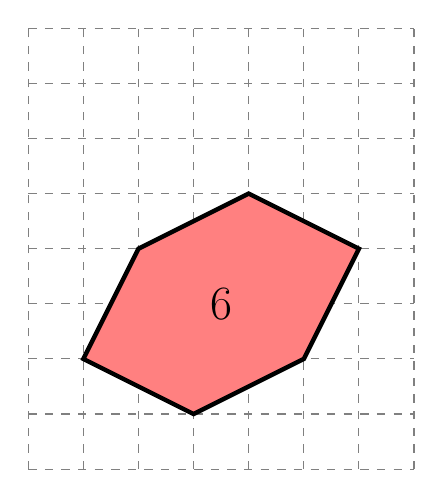
\begin{tikzpicture}[scale=0.7]
    \draw[gray, dashed] (0,0) grid (7,8);
    \draw[ultra thick, fill=red!50] (1,2)--(2,4)--(4,5)--(6,4)--(5,2)--(3,1)--cycle;
    \node at (3.5,3) {\LARGE 6};
  \end{tikzpicture}\hspace{1cm}
  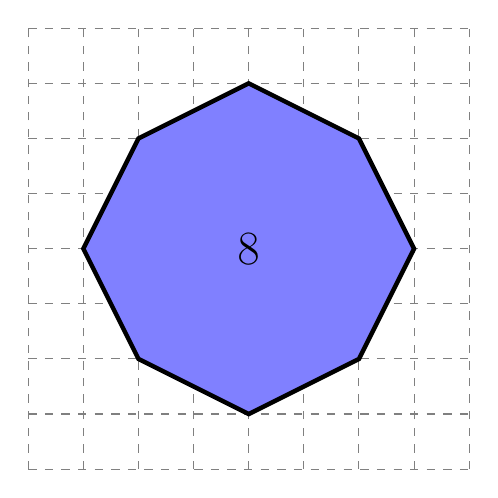
\begin{tikzpicture}[scale=0.7]
    \draw[gray, dashed] (0,0) grid (8,8);
    \draw[ultra thick, fill=blue!50] (2,2)--(1,4)--(2,6)--(4,7)--(6,6)--(7,4)--(6,2)--(4,1)--cycle;
    \node at (4,4) {\LARGE 8};
  \end{tikzpicture}
  \caption{
    Example demonstrating that $\ell_6 = \ell_8 = \sqrt{5}$.
  }
\end{figure}
\begin{question}
  For what values of $m$ do there exist equilateral $(2m-1)$-gons with integer
  coordinates?
\end{question}

\begin{related}
  \item For $m$ such that there are no equilateral $(2m-1)$-gons, what is do
    the best Diophantine approximations look like (in the sense of
    Problem 54)?
  \item Does this generalize to polyhedra?
\end{related}
\begin{references}
  \item \url{https://oeis.org/A071383}
  \item Problem 54
\end{references}
\end{document}
